\documentclass[10pt,slidestop]{beamer}
\synctex=1

\usepackage[T1]{fontenc}
\usepackage{amsmath,amssymb,amsopn}
\usepackage{mathtools}
\usepackage{booktabs}
\usepackage{array}
\usepackage{listings}
\usepackage{matlab-prettifier}
\usepackage{xcolor}
\usepackage{tikz}
\usetikzlibrary{arrows.meta,positioning,calc,shapes.geometric,fit,backgrounds}
\usepackage{algorithm}
\usepackage{algpseudocode}
\usepackage{ccicons}

\setlength{\parindent}{0pt}
\pdfcompresslevel=9

\definecolor{eclipseBlue}{RGB}{42,0,255}
\definecolor{eclipseGreen}{RGB}{63,127,95}
\definecolor{eclipsePurple}{RGB}{127,0,85}
\definecolor{codebg}{gray}{0.96}
\definecolor{darkblue}{RGB}{0,51,102}
\definecolor{darkgreen}{RGB}{0,102,51}
\definecolor{darkred}{RGB}{153,0,0}
\definecolor{orange}{RGB}{200,110,0}
\definecolor{lightblue}{RGB}{225,235,248}
\definecolor{lightgreen}{RGB}{223,242,223}
\definecolor{lightorange}{RGB}{252,238,220}

\lstset{
  basicstyle=\footnotesize\ttfamily,
  backgroundcolor=\color{codebg},
  frame=single, framesep=4pt,
  breaklines=true, showstringspaces=false,
  keywordstyle=\color{eclipsePurple}\bfseries,
  commentstyle=\color{eclipseGreen},
  stringstyle=\color{eclipseBlue},
}
\lstdefinestyle{ml}{style=Matlab-editor,basicstyle=\scriptsize\mlttfamily}

\setbeamertemplate{navigation symbols}{}
\setbeamertemplate{footline}{%
  \hfill\vspace*{1pt}\href{https://creativecommons.org/publicdomain/zero/1.0/}{\cczero}\hspace{.1cm}%
  \texttt{steady\_plan}\enspace--\enspace\insertframenumber/\inserttotalframenumber\enspace--\enspace\today\enspace}
\setbeamertemplate{blocks}[rounded][shadow=true]

\newcommand{\code}[1]{\texttt{#1}}
\newcommand{\ra}{$\rightarrow$}
\DeclareMathOperator{\SCC}{SCC}

\title{Deriving the steady state}
\subtitle{The \texttt{steady\_plan} algorithms}
\author{\texttt{stephane.adjemian@univ-lemans.fr}}
\date{modBuilder technical note --- \today}

\begin{document}

\begin{frame}\titlepage\end{frame}
\begin{frame}\frametitle{Outline}\tableofcontents\end{frame}

%==============================================================================
\section{The problem}
%==============================================================================

\begin{frame}\frametitle{Two routes to a steady state}
  \begin{columns}[t]
  \begin{column}{0.5\textwidth}
    \textbf{Write it}
    \begin{itemize}\small
    \item \code{steady(var, expr)} for each variable;
    \item you know the algebra, modBuilder carries it into the
      \code{steady\_state\_model} block;
    \item \code{checksteady} orders it, \code{write} emits it.
    \end{itemize}
  \end{column}
  \begin{column}{0.5\textwidth}
    \textbf{Derive it}
    \begin{itemize}\small
    \item \code{steady\_plan} reads the \emph{static structure} of the model;
    \item it pairs equations to variables, decomposes, and closes each block it
      can in closed form;
    \item \code{apply\_steady\_plan} writes the result out, generating a
      numerical routine for any block that resists.
    \end{itemize}
  \end{column}
  \end{columns}

  \vfill
  \begin{block}{This note}
    The algorithms behind the second route: the matching, the block
    decomposition, the closed-form recognisers, the gauge backout, and the
    diagnostics. Everything rests on the \code{ast} engine (companion note).
  \end{block}
\end{frame}

\begin{frame}\frametitle{The pipeline}
  \begin{center}
  \scalebox{0.92}{
  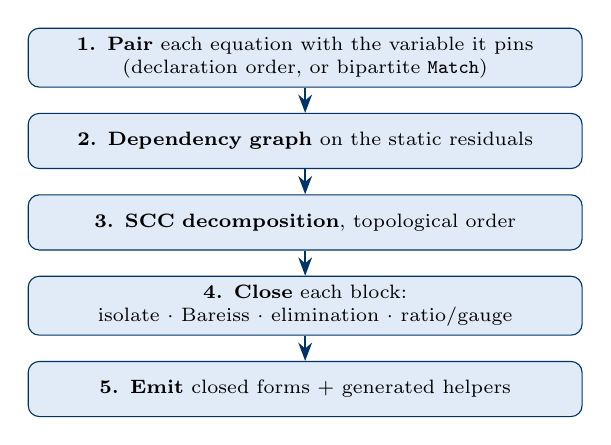
\begin{tikzpicture}[
    node distance=3.2mm,
    s/.style={rectangle,draw=darkblue,fill=lightblue,rounded corners,
      align=center,font=\scriptsize,text width=68mm,minimum height=7mm},
    a/.style={-{Stealth},darkblue,thick}]
    \node[s] (pair) {\textbf{1. Pair} each equation with the variable it pins\\
      (declaration order, or bipartite \code{Match})};
    \node[s,below=of pair] (dep) {\textbf{2. Dependency graph} on the static residuals};
    \node[s,below=of dep] (scc) {\textbf{3. SCC decomposition}, topological order};
    \node[s,below=of scc] (close) {\textbf{4. Close} each block:\\ isolate $\cdot$ Bareiss $\cdot$ elimination $\cdot$ ratio/gauge};
    \node[s,below=of close] (out) {\textbf{5. Emit} closed forms $+$ generated helpers};
    \draw[a](pair)--(dep); \draw[a](dep)--(scc); \draw[a](scc)--(close); \draw[a](close)--(out);
  \end{tikzpicture}}
  \end{center}
  \smallskip
  Options \code{Match}, \code{Anchors}, \code{PropagateKnown},
  \code{MaxBlockSize} steer stages 1, 4 and the known-value environment.
\end{frame}

%==============================================================================
\section{Pairing and decomposition}
%==============================================================================

\begin{frame}\frametitle{Equation--variable pairing}
  Each equation must be pinned to one endogenous variable. Two sources:

  \begin{itemize}
  \item \textbf{Declaration pairing} --- equation $i$ keeps the variable it was
    \code{add}ed with. Honours calibration swaps (an endogenous fixed by
    \code{calibrate} re-pairs its equation to the freed parameter).\newline
  \item \textbf{\code{Match=true}} --- recompute the pairing by bipartite
    matching on the \emph{simplified static residuals}. An arbitrary declaration
    pairing hides the recursive structure; matching exposes it, so a large
    simultaneous block usually falls apart into singletons plus a few small
    blocks.
  \end{itemize}

  \smallskip
  \begin{block}{Why the static residual}
    The dependency structure is invariant to leads/lags --- name equality is
    unchanged by \code{staticise}. So the whole analysis runs on the static
    residuals, and the recursive order it finds is the genuine steady-state
    order.
  \end{block}
\end{frame}

\begin{frame}\frametitle{Bipartite matching (\texttt{matchequations})}
  \begin{itemize}
  \item \textbf{Edge} $i \sim j$ iff variable $j$ appears in equation $i$
    \emph{and does not cancel} from its static residual --- tested by
    \code{ast.check\_factor} on \code{staticise().simplify()}. The cancellation
    filter is what keeps the matcher from pinning an equation to a variable that
    drops out at the steady state.\newline
  \item \textbf{Minimum-cost perfect matching} by \code{matchpairs}
    (Duff--Koster). Edge weights encode stable tie-breaks:
    \begin{enumerate}\small
    \item prefer a variable on the \textbf{LHS} of the equation;
    \item then prefer \textbf{rarer} candidates (Hall-style scarcity);
    \item then lexicographic by (equation, candidate).
    \end{enumerate}
  \item Exogenous driving processes and user anchors are removed from the
    candidate pool first, so the matcher cannot steal a shock variable to pin a
    real equation.
  \end{itemize}
\end{frame}

\begin{frame}\frametitle{Exogenous processes are anchors}
  A variable is \textbf{economically exogenous} when its equation references,
  among endogenous symbols, only variables of its own block (its own lags for an
  AR/ARMA, the block members for a VAR) \emph{and} the block is driven by an
  exogenous innovation.

  \begin{itemize}
  \item Such a block is a \textbf{sink} of the declaration-paired dependency
    graph --- nothing in the rest of the model determines it.\newline
  \item So its variables are free \textbf{anchors}: their steady-state level is
    not pinned by the model. They are excluded from the matching and solved
    first, each ARMA equation isolated for the level parameter it carries
    ($x = \bar x$).\newline
  \item \code{exogenous\_processes} detects them structurally --- no declaration
    needed. A multivariate (VAR) process is kept as one anchor block of size
    $>1$ and closed jointly, the determinant probe catching a unit root at the
    calibration.
  \end{itemize}
\end{frame}

\begin{frame}\frametitle{Dependency graph and SCC order}
  \begin{itemize}
  \item Build a directed graph on the paired variables: edge $j \to i$ iff
    $x_j$ is referenced by equation $i$ (and $j \neq i$).\newline
  \item \textbf{Strongly connected components} give the blocks:
    a cycle of mutual dependence is one simultaneous block; everything else is a
    singleton.\newline
  \item The \textbf{condensation} (one node per SCC) is a DAG; its topological
    sort is the evaluation order. In MATLAB: \code{conncomp(G,'Type','strong')}
    then \code{toposort} on the condensed graph.
  \end{itemize}

  \smallskip
  \begin{center}\scriptsize
  \begin{tabular}{@{}ll@{}}
    \toprule
    block \code{kind} & meaning \\
    \midrule
    \code{trivial} & one equation, variable not in its own residual \\
    \code{self-recursive} & one equation, variable in its own residual (a lag) \\
    \code{simultaneous} & SCC of size $>1$, jointly determined \\
    \code{anchor} & exogenous process / user normalisation \\
    \bottomrule
  \end{tabular}
  \end{center}
\end{frame}

%==============================================================================
\section{Closing blocks}
%==============================================================================

\begin{frame}\frametitle{Singletons: \texttt{isolate}}
  A block of one equation is closed by \code{ast.isolate} on its static
  residual --- the four recognisers of the companion note:

  \begin{enumerate}\small
  \item invertible call (\code{exp}/\code{log} wrapping the unknown),
  \item linear $a x + b = 0$,
  \item monomial $a x^d + b = 0$,
  \item binomial power $c_p x^p + c_q x^q = 0$,
  \end{enumerate}
  with a denominator-clearing retry.

  \medskip
  \begin{itemize}
  \item Success $\Rightarrow$ \code{closed\_form = \{var, expr\}}, plus a
    \textbf{knife-edge check}: evaluate \code{info.coefs} at the calibration; a
    pinning divisor that is symbolically non-zero but numerically zero is a unit
    root \emph{at this calibration}.\newline
  \item Failure with \code{info.unit\_root} (or the variable cancelling
    outright) $\Rightarrow$ the equation pins a growth rate, not a level: warn,
    the level is the modeller's to fix.
  \end{itemize}
\end{frame}

\begin{frame}\frametitle{Simultaneous blocks: three tiers}
  \code{close\_simultaneous} tries progressively more general machinery, gated
  by \code{MaxBlockSize} (default 8):

  \begin{enumerate}
  \item \textbf{Jointly linear} --- \code{linearise\_system} extracts
    $A x + b = 0$; \code{solve\_linear\_system} closes it by \textbf{Bareiss}
    triangulation $+$ back-substitution (fraction-free: entries stay
    polynomial). The determinant $\pm U_{nn}$ is the singularity probe.\newline
  \item \textbf{Iterated elimination} --- when not jointly linear:
    isolate one variable, substitute its closed form into every other equation,
    simplify, repeat. A consumed equation folds to $0=0$ and drops out.\newline
  \item \textbf{Ratio change of variables} --- last resort for a block that is
    homogeneous in its variables (next slides).
  \end{enumerate}

  \smallskip
  A stalled elimination reports the \textbf{reduced system} --- the still-open
  variables and their residuals with every closed form substituted in --- which
  is exactly what a generated helper will solve.
\end{frame}

\begin{frame}\frametitle{Homogeneous blocks pin ratios, not levels}
  Some blocks --- the Calvo price and wage recursions are the textbook case ---
  are \textbf{homogeneous} in their variables: every equation is invariant under
  a common rescaling. Their solution set is a ray through zero.

  \begin{itemize}
  \item Solving as-is would land on the trivial all-zero point. Both the linear
    path and elimination refuse (the rational normalisation rejects the zero
    ray).\newline
  \item \textbf{\code{ratio\_reduce}} --- if some equation involves the variables
    only through a ratio (homogeneous of degree 0, e.g. a factor-demand ratio
    $wL/rK=\text{const}$), write each variable as $\text{ratio}\cdot\text{gauge}$:
    the gauge cancels there, pinning the ratio, and the block reduces to a
    triangular system in $\{\text{ratios}, \text{gauge}\}$.\newline
  \item When the gauge does \emph{not} close internally ---
    its scale is pinned \emph{outside} the block --- \code{ratio\_parametrise}
    solves the ratios and returns each variable as $\text{ratio}\cdot\text{gauge}$,
    the gauge left free for the backout.
  \end{itemize}
\end{frame}

\begin{frame}\frametitle{The gauge backout}
  Freeing a normalisation anchor can leave a block homogeneous: its equations
  pin the ratios, and the \textbf{scale-pinning equation} (aggregate production,
  labour-market clearing) sits among the consistency conditions the anchors
  absorbed.

  \begin{center}
  \scalebox{0.9}{
  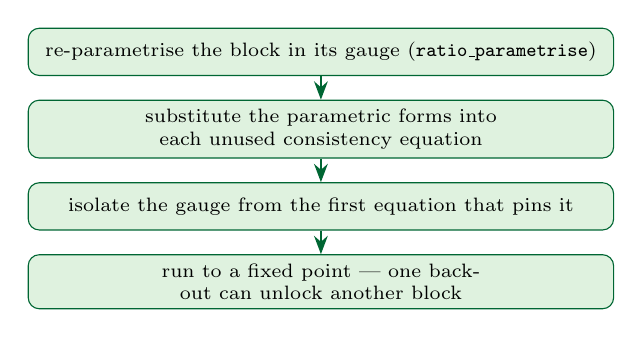
\begin{tikzpicture}[node distance=3mm,
    s/.style={rectangle,draw=darkgreen,fill=lightgreen,rounded corners,
      align=center,font=\scriptsize,text width=72mm,minimum height=6mm},
    a/.style={-{Stealth},darkgreen,thick}]
    \node[s] (p) {re-parametrise the block in its gauge (\code{ratio\_parametrise})};
    \node[s,below=of p] (sub) {substitute the parametric forms into each unused consistency equation};
    \node[s,below=of sub] (iso) {isolate the gauge from the first equation that pins it};
    \node[s,below=of iso] (fix) {run to a fixed point --- one backout can unlock another block};
    \draw[a](p)--(sub);\draw[a](sub)--(iso);\draw[a](iso)--(fix);
  \end{tikzpicture}}
  \end{center}

  \smallskip
  This is exactly the hand technique: solve in ratios, back the level out of a
  discarded equation. A multi-gauge block (several independent scales) re-matches
  and eliminates per gauge (\code{rematch\_eliminate}).
\end{frame}

%==============================================================================
\section{The known-value environment}
%==============================================================================

\begin{frame}\frametitle{\texttt{PropagateKnown}: folding what is known}
  Before the recognisers run, inline the values already known into the residuals:

  \begin{itemize}
  \item values declared through \code{steady()} (normalisations, markups, scales);
  \item the calibrated levels of the exogenous variables (innovations at 0).
  \end{itemize}

  \smallskip
  \begin{block}{Why it unlocks closures}
    Folding a shock to its level turns $\log(\text{shock})\to 0$ and
    $x/1 \to x$, collapsing factors that otherwise defeat the linear /
    invertible-call recognisers. A closed form that itself folds to a constant
    becomes known for the downstream blocks --- so
    \code{InflationFactor = InflationTarget} collapses to a parameter and
    linearises the price recursion.
  \end{block}

  \smallskip
  Only \emph{leaf} values (a number, a single symbol) are inlined --- inlining a
  full rental-rate formula would bloat the residual and defeat the recognisers.
\end{frame}

\begin{frame}\frametitle{Anchors and calibration swaps}
  Two ways to make an over- or under-determined static system square:

  \begin{block}{Normalisation anchors (\texttt{Anchors})}
    Endogenous variables whose level the modeller fixes (a scale, a
    symmetric-equilibrium normalisation). Each is removed from the matching;
    fixing $K$ anchors leaves $K$ equations unmatched --- the \textbf{consistency
    conditions} the anchor values must satisfy, which the gauge backout then
    consumes. A homogeneous (scale) normalisation is well-posed as is.
  \end{block}

  \begin{block}{Calibration swaps (\texttt{calibrate})}
    Pin an endogenous to a target, free a parameter to be solved instead ---
    count-neutral, so the system stays square. Pin hours to $1/3$, solve for the
    disutility weight; the labour FOC becomes linear in the weight, and the rest
    of the RBC reduces step by step.
  \end{block}
\end{frame}

%==============================================================================
\section{Blocks that resist}
%==============================================================================

\begin{frame}\frametitle{Generated numerical routines}
  A block the recognisers cannot close is \emph{not} abandoned to a global
  numerical solve. \code{apply\_steady\_plan(GenerateHelpers=true)} writes each
  such block to a self-contained routine \code{<base>\_ssblock\_<k>.m}:

  \begin{itemize}
  \item residuals and Jacobian inlined; the \code{steady\_state\_model} block
    gains the multi-output call
    \code{[x1,\dots,xn] = <base>\_ssblock\_<k>(deps\dots, params\dots)} at its
    topological position (Dynare accepts multi-output functions there).\newline
  \item The steady state stays analytical \emph{conditionally} on small numerical
    systems: analytic prologue, one small solve, analytic epilogue.\newline
  \item \code{Solver}: a damped Newton written into the file (self-contained), or
    delegate to \code{dynare\_solve} (\code{fsolve} via \code{solve\_algo=0}).
  \end{itemize}
\end{frame}

\begin{frame}\frametitle{The Jacobian by complex step}
  The generated routine's Jacobian (option \code{Jacobian='complex-step'} or
  \code{'auto'}) uses \textbf{complex-step differentiation}:
  \[
    f'(x) \;=\; \frac{\operatorname{Im} f(x + i h)}{h}, \qquad h = 10^{-20}.
  \]

  \begin{itemize}
  \item A finite difference $\tfrac{f(x+h)-f(x)}{h}$ is capped by
    \textbf{catastrophic cancellation}: $f(x+h)$ and $f(x)$ share leading digits
    that subtract away, so $h$ cannot be made small.\newline
  \item The complex step takes the step in the \emph{imaginary} direction. For
    analytic $f$, the imaginary part of $f(x+ih)$ carries $h f'(x)$ with
    \textbf{no subtraction} --- exact to machine precision, and $h$ can be tiny.\newline
  \item Requires only that the block's residuals use complex-analytic operators;
    \code{'auto'} checks this and falls back to the inlined symbolic derivative
    otherwise.
  \end{itemize}
\end{frame}

%==============================================================================
\section{Diagnostics and suggestions}
%==============================================================================

\begin{frame}\frametitle{Three unit-root diagnostics}
  \code{steady\_plan} distinguishes three ways a level fails to be pinned:

  \begin{itemize}\small
  \item \code{unitRoot} --- an AR-type equation whose coefficients on the
    recurring term cancel in the static residual ($\log Z = \log Z(-1) + e$):
    pins the \textbf{growth rate}. Declare the level or pass an anchor.\newline
  \item \code{endogenousUnitRoot} --- an equation pins \emph{none} of the
    remaining variables; its static residual reduces to a condition on parameters
    (the Euler condition $1 - \beta R = 0$ of an incomplete-markets economy). A
    level is set by initial conditions, not the model. Close the model
    (debt-elastic premium, endogenous discounting).\newline
  \item \code{calibrationUnitRoot} --- symbolically regular but singular
    \emph{at the calibrated point}: a pinning coefficient ($1-R$ at $R=1$) or a
    block determinant ($1-k^2$ at $k=1$) evaluates to zero, so a closed form
    divides by a numerical zero. Move the calibration off the knife edge.
  \end{itemize}
\end{frame}

\begin{frame}\frametitle{Scale symmetries}
  \code{scaling\_symmetries} finds the scale freedoms of the steady-state system
  directly: exponents $(e_1,\dots,e_n)$ on the variables such that a joint
  rescaling $x_i \mapsto \lambda^{e_i} x_i$ leaves every static equation
  homogeneous.

  \begin{itemize}
  \item Each independent symmetry is a scale freedom; its invariant ratios
    ($K/L$, $C/Y$) are the intensive variables that make the system scale-free.\newline
  \item Diagnostic only --- it reports the co-scaling groups and their exponents,
    it does not rewrite the model.\newline
  \item With \code{IncludeParameters=true}, level parameters may scale too,
    revealing the latent structure that explicit normalisation parameters
    otherwise pin.
  \end{itemize}

  \smallskip
  This is the structural explanation of \emph{why} a homogeneous block needs a
  gauge: a scale symmetry is a direction the equations do not constrain.
\end{frame}

\begin{frame}\frametitle{Reducing and finding anchors}
  \begin{block}{\texttt{suggest\_anchors} --- fewer knowns}
    Greedy leave-one-out to a fixed point: a declared anchor is dropped when the
    plan closes just as well without its anchor status \emph{and} its value. It
    never invents a value --- it reports which of the declared knowns the
    structure actually needs. (This is how the Smets--Wouters example was reduced
    from 23 anchors to 7.)
  \end{block}

  \begin{block}{\texttt{suggest\_calibrations} --- close a residual}
    For each still-open variable, scan the parameters in its equation; virtually
    apply each \code{(endo, param)} swap (\code{copy} $+$ \code{calibrate},
    re-plan) and record the new residual. Returns only swaps that strictly
    shrink it, full closures first. The menu is algebraic --- read it critically,
    then apply with \code{calibrate}. \code{print\_steady\_plan} prints it
    automatically when a plan stalls.
  \end{block}
\end{frame}

%==============================================================================
\section{Summary}
%==============================================================================

\begin{frame}\frametitle{Summary}
  \begin{itemize}
  \item Pair equations to variables (declaration or bipartite \code{Match}),
    excluding exogenous processes and anchors.\newline
  \item Decompose the static dependency graph into SCCs, evaluate in topological
    order.\newline
  \item Close each block: \code{isolate} for singletons; Bareiss, iterated
    elimination, or the ratio/gauge machinery for simultaneous ones; a generated
    complex-step routine for what resists.\newline
  \item \code{PropagateKnown} folds knowns to unlock closures; anchors and
    calibration swaps square the system.\newline
  \item Diagnostics separate genuine unit roots, incomplete models and
    knife-edge calibrations; \code{suggest\_*} propose the minimal knowns or the
    closing swap.
  \end{itemize}

  \vfill
  \centering\small Reference: the Steady-State Analysis section of
  \texttt{README.md}, the \texttt{examples/} models, and the \texttt{steady\_plan}
  docstrings.
\end{frame}

\end{document}
